\documentclass[gr-notes.tex]{subfiles}

\begin{document}

\setcounter{chapter}{2}

\chapter{Tensor analysis in special relativity}



\setcounter{section}{2}

\section{The $\binom{0}{1}$ tensors: one-forms}

The symbol $\tilde{}$ is used to denote a one-form, as $\vec{}$ is used to denote a vector. So $\tilde{p}$ is a one-form, or a type $\binom{0}{1}$ tensor.



\subsection*{Normal one-forms}

Let $\mathcal{S}$ be some surface.

$\forall \vec{V}$ tangent to $\mathcal{S}$, $\tilde{p}(\vec{V}) = 0 \implies \tilde{p}$ is normal to $\mathcal{S}$.

Furthermore, if $\mathcal{S}$ is a \emph{closed} surface \& $\tilde{p}$ is normal to $\mathcal{S}$ \& $\forall \vec{U}$ pointing outwards from $\mathcal{S}$, $\tilde{p}(\vec{U}) > 0 \implies \tilde{p}$ is an outward normal one-form.



\setcounter{section}{4}

\section{Metric as a mapping of vectors into one-forms}

\subsection*{Normal vectors and unit normal one-forms}

$\vec{V}$ is normal to a surface if $\tilde{V}$ is normal to the surface. They are said to be \emph{unit normal} if their magnitude is $\pm 1$, so $\vec{V}^2 = \tilde{V}^2 = \pm 1$.

\begin{itemize}
\item A time-like unit normal has magnitude $-1$
\item A space-like unit normal has magnitude $+1$
\item A null normal cannot be a unit normal, because $\vec{V}^2 = \tilde{V}^2 = 0$
\end{itemize}



\setcounter{section}{9}

\section{Exercises}

\textbf{3}

(a)
\begin{align*}
  \tilde{p}(A^\alpha \vec{e}_\alpha) &=
  A^\alpha \tilde{p}(\vec{e}_\alpha) =
  \tilde{p}(A^0 \vec{e}_0 + A^1 \vec{e}_1 + A^2 \vec{e}_2 + A^3 \vec{e}_3)
  \\ &=
  A^0 \tilde{p}(\vec{e}_0) + A^1 \tilde{p}(\vec{e}_1 +
  A^2 \tilde{p}(\vec{e}_2) + A^3 \tilde{p}(\vec{e}_3 =
  A^\alpha \tilde{p}(\vec{e}_\alpha) = A^\alpha p_\alpha \in \mathbb{R}
\end{align*}

(b)

\begin{align*}
  \tilde{p} &\underset{\obs}{\to} (-1, 1, 2, 0)
  \\
  \vec{A}   &\underset{\obs}{\to} (2, 1, 0, -1)
  \\
  \vec{B}   &\underset{\obs}{\to} (0, 2, 0, 0)
\end{align*}

\begin{align*}
  \tilde{p}(\vec{A}) &=
  -2 + 1 + 0 + 0 = -1
  \\
  \tilde{p}(\vec{B}) &=
  0 + 2 + 0 + 0 = 2
  \\
  \tilde{p}(\vec{A} - 3 \vec{B}) &=
  \tilde{p}(\vec{A}) - 3 \tilde{p}(\vec{B}) =
  -1 - 3 \cdot 2 = -7
\end{align*}

\textbf{4}
Given the following vectors
\begin{align*}
  \vec{A} & \underset{\obs}{\to} ( 2, 1, 1, 0) &
  \vec{B} & \underset{\obs}{\to} ( 1, 2, 0, 0) \\
  \vec{C} & \underset{\obs}{\to} ( 0, 0, 1, 1) &
  \vec{D} & \underset{\obs}{\to} (-3, 2, 0, 0)
\end{align*}

(Note that all parts were done with the assistance of \texttt{numpy}.)

(a) Show that they are linearly independent.

We do this by constructing a matrix, $\vb{X}$, whose columns correspond to the four vectors. If the determinant of $\vb{X}$ is non-zero, then that means the vectors are linearly independent.
%
\begin{displaymath}
  \det(\vb{X}) =
  \det \mqty(2 &  1 &  0 & -3 \\
             1 &  2 &  0 &  2 \\
             1 &  0 &  1 &  0 \\
             0 &  0 &  1 &  0) =
  -8
\end{displaymath}

(b) Find the components of $\tilde{p}$ if
%
\begin{displaymath}
  \tilde{p}(\vec{A}) =  1, \quad
  \tilde{p}(\vec{B}) = -1, \quad
  \tilde{p}(\vec{C}) = -1, \quad
  \tilde{p}(\vec{D}) =  0
\end{displaymath}

We do this by observing that $\tilde{p} = A^\alpha p_\alpha$, and so we have a system of four equations, which we can write in matrix form as
%
\begin{align*}
  \mqty( \vec{A} \\ \vec{B} \\ \vec{C} \\ \vec{D} ) \tilde{p} &=
  \mqty( 1 \\ -1 \\ -1 \\ 0 )
  \\ \implies
  \tilde{p} &=
  \mqty( \vec{A} \\ \vec{B} \\ \vec{C} \\ \vec{D} )^{-1}
  \mqty( 1 \\ -1 \\ -1 \\ 0 )
  \\ &=
  \mqty( -\frac{1}{4} \\ -\frac{3}{8} \\ +\frac{15}{8} \\ -\frac{23}{8} ).
\end{align*}

(c) Find $\tilde{p}(\vec{E})$, where $\vec{E} \to_\obs (1, 1, 0, 0)$.

\begin{displaymath}
  \tilde{p}(\vec{E}) = p_\alpha E^\alpha = -\frac{5}{8}
\end{displaymath}

(d) Determine whether $\tilde{p}$, $\tilde{q}$, $\tilde{r}$, and $\tilde{s}$ are linearly independent.

We do this by first setting up a system of equations for each of $\tilde{q}$, $\tilde{r}$, and $\tilde{s}$, as was done for $\tilde{p}$, and solving. I will refer to the matrix whose rows were $\vec{A}$, $\vec{B}$, $\vec{C}$, and $\vec{D}$ as $\vb{X}$.
%
\begin{align*}
  \vb{X} \tilde{q} &= \mqty( +0 \\ +0 \\ +1 \\ -1 ) &
  \vb{X} \tilde{r} &= \mqty( +2 \\ +0 \\ +0 \\ +0 ) &
  \vb{X} \tilde{s} &= \mqty( -1 \\ -1 \\ +0 \\ +0 )
  \\
  \tilde{q} &=
  \mqty( +\frac{1}{4} \\ -\frac{1}{8} \\ -\frac{3}{8} \\ +\frac{11}{8} ) &
  \tilde{r} &=
  \mqty( +0 \\ +0 \\ +2 \\ +2 ) &
  \tilde{s} &=
  \mqty( -\frac{1}{4} \\ -\frac{3}{8} \\ -\frac{1}{8} \\ +\frac{1}{8} )
\end{align*}
%
Now if the matrix whose columns are comprised of $\tilde{p}$, $\tilde{q}$, $\tilde{r}$, and $\tilde{s}$ has a non-zero determinant, then the four covectors must be linearly independent.
%
\begin{displaymath}
  \det \mqty( \tilde{p} & \tilde{q} & \tilde{r} & \tilde{s} ) = \frac{1}{4},
\end{displaymath}
%
and so they are indeed linearly independent.


\textbf{6}

(a) Show that $\tilde{p} \neq \tilde{p}(\vec{e}_\alpha) \tilde{\lambda}^\alpha$ for arbitrary $\tilde{p}$.

Let us choose $\tilde{p} \to_\obs (0, 1, e, \pi)$, as a counter-example.
%
\begin{align*}
  p_\alpha \tilde{\lambda}^\alpha &\underset{\obs}{\to}
  0 \cdot (1, 1, 0, 0) +
  1 \cdot (1, -1, 0, 0) +
  e \cdot (0, 0, 1, -1) +
  \pi \cdot (0, 0, 1, 1)
  \\ &\underset{\obs}{\to}
  (1, -1, e+\pi, 0)
  \underset{\obs}{\cancel\to}
  \tilde{p}
\end{align*}

(b) $\tilde{p} \to_\obs (1, 1, 1, 1)$. Find $l_\alpha$ such that
%
\begin{displaymath}
  \tilde{p} = l_\alpha \tilde{\lambda}^\alpha
\end{displaymath}

We may do this with a simple matrix inversion. We define $\vb\Lambda$ to be the matrix whose rows are formed by $\tilde{\lambda}^\alpha$.
%
\begin{displaymath}
  \vb\Lambda l = p \implies
  l = \vb\Lambda^{-1} p =
  \mqty( 1 \\ 0 \\ 1 \\ 0 )
\end{displaymath}




\textbf{8}
Draw the basis one-forms $\tilde{\dd}t$ and $\tilde{\dd}x$ of frame $\obs$.

They are
%
\begin{align*}
  \tilde{\dd}t &\underset{\obs}{\to} (1, 0, 0, 0), \\
  \tilde{\dd}x &\underset{\obs}{\to} (0, 1, 0, 0),
\end{align*}
%
and they are shown in Figure \ref{fig:ch3-problem-8}.

\begin{figure}[h]
  \centering
  \includegraphics[width=0.75\textwidth]{img/ch3_problem_8}
  \caption{Problem 8: Basis one-forms of $\obs$. $\tilde{\dd}t$ is given in blue and $\tilde{\dd}x$ in red.}
  \label{fig:ch3-problem-8}
\end{figure}


\textbf{9}
At the points $\mathcal{P}$ and $\mathcal{Q}$, estimate the components of the gradient $\tilde{\dd}T$.

Recall that $\tilde{\dd}T \to_\obs \qty(\pdv{T}{x}, \pdv{T}{y})$, and so $\Delta T = \tilde{\dd}T_\alpha x^\alpha = \tilde{\dd}T_x \Delta x + \tilde{\dd}T_y \Delta y$.

Now if we move only in the $x$ direction from one of the points, we move some distance $\Delta x$, change our temperature by $\Delta t$, and $\Delta y = 0$. Likewise for a movement in the $y$ direction. Thus we can say
%
\begin{align*}
  \Delta T &= \tilde{\dd}T_x \Delta x &
  \Delta T &= \tilde{\dd}T_y \Delta y
  \\
  \tilde{\dd}T_x &= \frac{\Delta T}{\Delta x} &
  \tilde{\dd}T_y &= \frac{\Delta T}{\Delta y}
\end{align*}
%
In Figure \ref{fig:ch3-problem-9}, from $\mathcal{P}$ I move a distance $\Delta x = 0.5$, which causes a temperature change of $\Delta T = -7$, giving $\tilde{\dd}T_x = -14$. Then I move a distance $\Delta y = 0.5$ and get the same temperature change of $\Delta T = -7$, and so I conclude that at point $\mathcal{P}$, $\tilde{\dd}T \to_\obs (-14, -14)$.

At $\mathcal{Q}$, we are in a flat region where $T = 0$. If we move any non-zero distance $\Delta x$ or $\Delta y$, so long as it does not cross the $T = 0$ isotherm, we have a $\Delta T = 0$, and thus $\tilde{\dd}Tp \to_\obs (0, 0)$.

\begin{figure}[h]
  \centering
  \includegraphics[width=0.75\textwidth]{img/ch3_problem_9}
  \caption{Problem 9: Isotherms.}
  \label{fig:ch3-problem-9}
\end{figure}


\textbf{13}
Prove that $\tilde{\dd}f$ is normal to surfaces of constant $f$.

If we move some small distance $\Delta x^\alpha = \epsilon$, then there will be no change in the value of $f$, and thus we can say $\pdv*{f}{x^\alpha} = 0$, so
%
\begin{displaymath}
  \tilde{\dd}f =
  \pdv{f}{x^\alpha} \tilde{\dd}x^\alpha =
  0 \tilde{\dd}x^\alpha =
  0.
\end{displaymath}
%
Since $\tilde{\dd}f$ is defined to be normal to a surface if it is zero on every tangent vector, we have shown that $\tilde{\dd}f$ is normal to any surface of constant $f$.



\textbf{14}

\begin{align*}
  \tilde{p} &\underset{\obs}{\to} ( 1, 1, 0, 0) &
  \tilde{q} &\underset{\obs}{\to} (-1, 0, 1, 0)
\end{align*}

Prove by giving two vectors $\vec{A}$ and $\vec{B}$ as arguments that $\tilde{p} \otimes \tilde{q} \neq \tilde{q} \otimes \tilde{p}$. Then find the components of $\tilde{p} \otimes \tilde{q}$.

\begin{align*}
  (\tilde{p} \otimes \tilde{q})(\vec{A}, \vec{B}) &=
  \tilde{p}(\vec{A}) \tilde{q}(\vec{B}) =
  A^\alpha p_\alpha B^\beta q_\beta =
  (A^0 + A^1) (-B^0 + B^2),
  \\ &=
  -A^0 B^0 + A^0 B^2 - A^1 B^0 + A^1 B^2
  \\
  (\tilde{q} \otimes \tilde{p})(\vec{A}, \vec{B}) &=
  \tilde{q}(\vec{A}) \tilde{p}(\vec{B}) =
  A^\alpha q_\alpha B^\beta p_\beta =
  (-A^0 + A^2) (B^0 + B^1)
  \\ &=
  -A^0 B^0 - A^0 B^1 + A^2 B^0 + A^2 B^1,
\end{align*}
%
And so we see that $\otimes$ is not commutative.

The components of the outer product of two tensors are given by the products of the components of the individual tensors. Thus we can write the components as a $4 \times 4$ matrix.
%
\begin{displaymath}
  (\tilde{p} \otimes \tilde{q})_{\alpha\beta} =
  p_\alpha q_\beta =
  \mqty(-1 &  0 &  1 &  0 \\
        -1 &  0 &  1 &  0 \\
         0 &  0 &  0 &  0 \\
         0 &  0 &  0 &  0)
\end{displaymath}




\textbf{18}

(a)
Find the one-forms mapped by $\vb{g}$ from
%
\begin{align*}
  \vec{A} &\underset{\obs}{\to} ( 1,  0, -1,  0), &
  \vec{B} &\underset{\obs}{\to} ( 0,  1,  1,  0), \\
  \vec{C} &\underset{\obs}{\to} (-1,  0, -1,  0), &
  \vec{D} &\underset{\obs}{\to} ( 0,  0,  1,  1).
\end{align*}

In general,
%
\begin{displaymath}
  \vec{V} \underset{\obs}{\to} (V^0, V^1, V^2, V^3) \implies
  \tilde{V} =
  \vb{g} \vec{V} \underset{\obs}{\to} (-V^0, V^1, V^2, V^3),
\end{displaymath}
%
and so
%
\begin{align*}
  \tilde{A} &\underset{\obs}{\to} (-1,  0, -1,  0), &
  \tilde{B} &\underset{\obs}{\to} ( 0,  1,  1,  0), \\
  \tilde{C} &\underset{\obs}{\to} ( 1,  0, -1,  0), &
  \tilde{D} &\underset{\obs}{\to} ( 0,  0,  1,  1).
\end{align*}

(b)
Find the vectors mapped by $\vb{g}$ from
%
\begin{align*}
  \tilde{p} &\underset{\obs}{\to} ( 3,  0, -1, -1), &
  \tilde{q} &\underset{\obs}{\to} ( 1, -1,  1,  1), \\
  \tilde{r} &\underset{\obs}{\to} ( 0, -5, -1,  0), &
  \tilde{s} &\underset{\obs}{\to} (-2,  1,  0,  0).
\end{align*}
%
By using the inverse tensor in reverse, we have the same effect as before, of negating the first component
%
\begin{align*}
  \vec{p} &\underset{\obs}{\to} (-3,  0, -1, -1), &
  \vec{q} &\underset{\obs}{\to} (-1, -1,  1,  1), \\
  \vec{r} &\underset{\obs}{\to} ( 0, -5, -1,  0), &
  \vec{s} &\underset{\obs}{\to} ( 2,  1,  0,  0).
\end{align*}


\textbf{20}

In Euclidean 3-space, vectors and covectors are usually treated as the same, because they transform the same. We will now prove this.


(a)
Show that $A^{\bar\alpha} = \tensor{\Lambda}{^{\bar\alpha}_\beta} A^\beta$ and $P_{\bar\beta} = \tensor{\Lambda}{^{\alpha}_{\bar\beta}} P_\alpha$ are the same transformations if $\{ \tensor{\Lambda}{^{\alpha}_{\bar\beta}} \}$ is equal to the transpose of its inverse.

We can write that last statement as
%
\begin{displaymath}
  \tensor{\Lambda}{^{\alpha}_{\bar\beta}} =
  ((\tensor{\Lambda}{^{\alpha}_{\bar\beta}})^{-1})^T
\end{displaymath}
%
and we know that
%
\begin{displaymath}
  (\tensor{\Lambda}{^{\alpha}_{\bar\beta}})^{-1} =
  \tensor{\Lambda}{^{\bar\beta}_{\alpha}},
\end{displaymath}
%
and also we know that the Lorentz transformation is symmetric, and so
%
\begin{displaymath}
  (\tensor{\Lambda}{^{\bar\beta}_{\alpha}})^T =
  \tensor{\Lambda}{^{\bar\beta}_{\alpha}},
\end{displaymath}
%
which leads us to conclude that $\tensor{\Lambda}{^{\alpha}_{\bar\beta}} = \tensor{\Lambda}{^{\bar\beta}_{\alpha}}$, meaning the two transformations are the same.

(b)
The metric has components $\{ \delta_{ij} \}$. Prove that transformations between Cartesian coordinate systems must satisfy
\begin{displaymath}
  \delta_{\bar{i}\bar{j}} =
  \tensor{\Lambda}{^k_{\bar{i}}}
  \tensor{\Lambda}{^l_{\bar{j}}}
  \delta_{kl},
\end{displaymath}
and that this implies that $\tensor{\Lambda}{^k_{\bar{i}}}$ is an orthogonal matrix.

\begin{displaymath}
  \delta_{\bar{i}\bar{j}} =
  \vb{g}(\vec{e}_{\bar{i}}, \vec{e}_{\bar{j}}) =
  \vb{g}(\tensor{\Lambda}{^k_{\bar{i}}} \vec{e}_k,
         \tensor{\Lambda}{^l_{\bar{j}}} \vec{e}_j) =
  \tensor{\Lambda}{^k_{\bar{i}}}
  \tensor{\Lambda}{^l_{\bar{j}}}
  \vb{g}(\vec{e}_k, \vec{e}_j) =
  \tensor{\Lambda}{^k_{\bar{i}}}
  \tensor{\Lambda}{^l_{\bar{j}}}
  \delta_{kl}
\end{displaymath}

\textbf{Now show it is orthogonal}


\textbf{21}

(a) A region of the $t$--$x$ plane is bounded by lines $t=0$, $t=1$, $x=0$, and $x=1$. Within the plane, find the unit outward normal 1-forms and their vectors for each boundary line.

I define unit outward normals as follows:

Let $\mathcal{S}$ be a closed surface. If, for each $\vec{V}$ tangent to $\mathcal{S}$, we have $\tilde{p}(\vec{V}) = 0$, then $\tilde{p}$ is normal to $\mathcal{S}$.

In addition, if, for each $\vec{U}$ which points outwards from the surface, we have $\tilde{p}(\vec{U}) > 0$, then $\tilde{p}$ is an outward normal.

Furthermore, if $\tilde{p}^2 = \pm 1$, then it is a unit outward normal.

For the problem at hand, I define the region inside the four lines to be \emph{Inside}, and the region outside to be \emph{Outside}. For each of the four lines, I draw a vector $\vec{V}$ tangent (parallel) to the line, and $\vec{U}$ pointing outwards (See Figure \ref{fig:ch3-problem-21a}).

It helps to look at $t = 0$ and $t = 1$ together, and likewise for $x$, so I will start with $t$. We start with an arbitrary $\tilde{p} \to_\obs (p_0, p_1)$, and $\vec{V} \to_\obs (0, V^1)$, where $V^1 \neq 0$.
\begin{displaymath}
  \tilde{p}(\vec{V}) =
  p_0 \cdot 0 + p_1 V^1 = 0
  \implies
  p_1 = 0,
\end{displaymath}
so $\tilde{p} \to_\obs (p_0, 0)$ is a normal 1-form to both lines. Now we find the corresponding \emph{unit} normal, by taking
\begin{displaymath}
  \tilde{p}^2 = \pm 1 = -(p_0)^2 \implies
  \tilde{p}^2 = -1 \ \& \ p_0 = \pm 1.
\end{displaymath}

Whether we choose $p_0$ to be positive or negative now depends on the line we are looking at, and which direction is outward. For $t = 0$, we have a vector $\vec{U} = (-U^0, U^1)$, where $U^0 > 0$.
\begin{displaymath}
  \tilde{p}(\vec{U}) =
  p_0 (-U^0) + 0 \cdot U^1 > 0
  \implies
  -p_0 U^0 > 0
  \implies
  p_0 < 0,
\end{displaymath}
so for $t = 0$ we have $\tilde{p} \to_\obs (-1, 0)$, and likewise for $t = 1$ we have $\tilde{p} \to_\obs (1, 0)$. To get the associated \emph{vectors}, we apply the metric $\eta^{\alpha\beta}$, giving us $\vec{p} \to_\obs (1, 0)$ for $t = 0$ and $\vec{p} \to_\obs (-1, 0)$ for $t = 1$.

For $x = 0$ and $x = 1$, we instead have $\vec{V} \to_\obs (V^0, 0)$, and following the same steps as before, we conclude that: for $x = 0$, $\tilde{p} \to_\obs (0, -1)$, $\vec{p} \to_\obs (0, -1)$, and for $x = 1$, $\tilde{p} \to_\obs (0, 1)$, $\vec{p} \to_\obs (0, 1)$.

\begin{figure}[h]
  \centering
  
  \caption{Problem 21.a}
  \label{fig:ch3-problem-21a}
\end{figure}

(b)
Let another region be bounded by the set of points $\{ (1,0),(1,1),(2,1) \}$. Find an outward normal for the null boundary and the associated vector.




\textbf{23}

(a)
Prove that the set of all $\binom{M}{N}$ tensors forms a vector space, $V$.

Let $T$ be the set of all $\binom{M}{N}$ tensors, $\vb{s}, \vb{p}, \vb{q} \in T$, $\vec{A} \in \mathbb{R}^n$, and $\alpha \in \mathbb{R}$. For $T$ to be a vector space, we must define the operations of addition, and scalar multiplication (amongst others).

\textbf{Addition:}
\begin{displaymath}
  \vb{s} = \vb{p} + \vb{q} \implies
  \vb{s}(\vec{A}) = \vb{p}(\vec{A}) + \vb{q}(\vec{A})
\end{displaymath}

\textbf{Scalar Multiplication:}
\begin{displaymath}
  \vb{r} = \alpha \vb{p} \implies
  \vb{r}(\vec{A}) = \alpha \vb{p}(\vec{A})
\end{displaymath}


(b)

Prove that a basis for $T$ is
\begin{displaymath}
  \{ \vec{e}_\alpha \otimes \ldots \otimes \vec{e}_\gamma
     \otimes
     \tilde{\omega}^\mu \otimes \ldots \otimes \tilde{\omega}^\lambda \}
\end{displaymath}

\textbf{Still working on it}


\textbf{24}
Given:
\begin{displaymath}
  M^{\alpha\beta} \to
  \mqty(
     0 &  1 &  0 &  0 \\
     1 & -1 &  0 &  2 \\
     2 &  0 &  0 &  1 \\
     1 &  0 & -2 &  0
  )
\end{displaymath}


(a)
Find:

(i)
\begin{displaymath}
  M^{(\alpha\beta)} \to
  \mqty(
    0 & 1 & 1 & \frac{1}{2} \\
    1 & -1 & 0 & 1 \\
    1 & 0 & 0 & -\frac{1}{2} \\
    \frac{1}{2} & 1 & -\frac{1}{2} & 0
  );
  \quad
  M^{[\alpha\beta]} \to
  \mqty(
    0 & 0 & -1 & -\frac{1}{2} \\
    0 & 0 & 0 & 1 \\
    1 & 0 & 0 & \frac{3}{2} \\
    \frac{1}{2} & -1 & -\frac{3}{2} & 0
  )
\end{displaymath}


(ii)
\begin{displaymath}
  \tensor{M}{^\alpha_\beta} =
  \tensor{\eta}{_{\beta\mu}} \tensor{M}{^{\alpha\mu}} \to
  \mqty(
    0 & -1 & 0 & 0 \\
    1 & -1 & 0 & 2 \\
    2 & 0 & 0 & 1 \\
    1 & 0 & -2 & 0
  )
\end{displaymath}


(iii)
\begin{displaymath}
  \tensor{M}{_\alpha^\beta} =
  \tensor{\eta}{_{\alpha\mu}} \tensor{M}{^{\mu\beta}} \to
  \mqty(
    0 & -1 & 0 & 0 \\
    1 & -1 & 0 & 2 \\
    2 & 0 & 0 & 1 \\
    1 & 0 & -2 & 0
  )
\end{displaymath}


(iv)
\begin{displaymath}
  \tensor{M}{_{\alpha\beta}} =
  \tensor{\eta}{_{\beta\mu}} \tensor{M}{_\alpha^\mu} \to
  \mqty(
     0 &  1 &  0 &  0 \\
     1 & -1 &  0 &  2 \\
     2 &  0 &  0 &  1 \\
     1 &  0 & -2 &  0
  )
\end{displaymath}

(b) Does it make sense to separate the $\binom{1}{1}$ tensor with components $\tensor{M}{^\alpha_\beta}$ into symmetric and antisymmetric parts?

No, it would not make sense. For one, the notation for (anti)symmetric tensors do not even allow one to write it sensibly ($\tensor{M}{^{(\alpha}_{\beta)}}$). More importantly, one argument refers to vectors, and the other to covectors, so it does not make sense to switch them.

(c)

\begin{displaymath}
  \tensor{\eta}{^\alpha_\beta} =
  \tensor{\eta}{^{\alpha\mu}} \tensor{\eta}{_{\beta\mu}} =
  \mqty(\dmat[0]{-1,1,1,1}) \mqty(\dmat[0]{-1,1,1,1}) =
  \mqty(\imat{4}) =
  \tensor{\delta}{^\alpha_\beta}
\end{displaymath}





\textbf{31}

\textbf{Still working on it}



(\textbf{33})


\textbf{34}
Define double-null coordinates $u = t-x$, $v = t + x$ in Minkowski space.

(a)
Let $\vec{e}_u$ be the vector connecting the $(u,v,y,t)$ coordinates $(0,0,0,0)$ and $(1,0,0,0)$, and let $\vec{e}_v$ be the vector connecting $(0,0,0,0)$ and $(0,1,0,0)$. Find $\vec{e}_u$ and $\vec{e}_v$ in terms of $\vec{e}_t$ and $\vec{e}_x$, and plot the basis vectors in a spacetime diagram of the $t$--$x$ plane.

\begin{align*}
  u &= t - x = 0 \implies t =  +x &
  v &= t + x = 0 \implies t =  -x
  \\
  u &= t - x = 1 \implies t = 1+x &
  v &= t + x = 1 \implies t = 1-x &
\end{align*}

We draw the vectors $\vec{e}_u$ and $\vec{e}_v$ in Figure \ref{fig:ch3-problem-34a}, such that they point from the appropriate points of intersection on these lines of constant $u$ and $v$. From this it is obvious that $\vec{e}_v + \vec{e}_u = \vec{e}_t$, and that $\vec{e}_v - \vec{e}_u = \vec{e}_x$, or likewise $\vec{e}_v = \vec{e}_t - \vec{e}_u$ and $\vec{e}_u = \vec{e}_v - \vec{e}_x$. This is a system of 2 equations with two unknowns.

\begin{align*}
  \vec{e}_v &=
  \vec{e}_t - \vec{e}_v + \vec{e}_x \implies &
  \vec{e}_v &=
  \frac{1}{2} (\vec{e}_t + \vec{e}_x),
  \\
  \vec{e}_u &=
  \frac{1}{2} (\vec{e}_t + \vec{e}_x) - \vec{e}_x \implies &
  \vec{e}_u &=
  \frac{1}{2} (\vec{e}_t - \vec{e}_x).
\end{align*}

\begin{figure}[b]
  \centering
  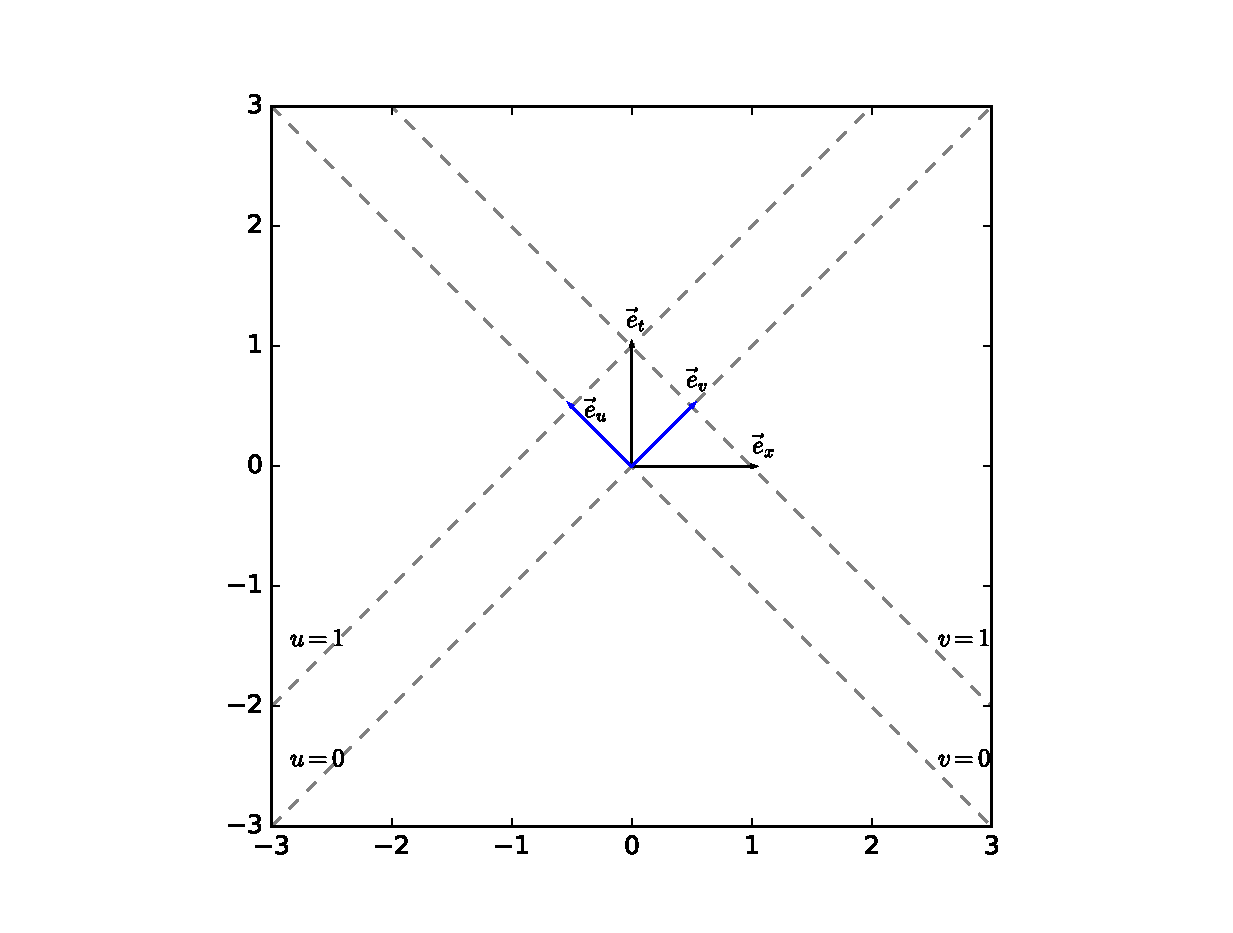
\includegraphics[width=0.75\textwidth]{img/ch3_problem_34a}
  \caption{Problem 34a: Spacetime diagram of double-null coordinate basis
    vectors in $t$--$x$ plane.}
  \label{fig:ch3-problem-34a}
\end{figure}

(b)
Show that $\vec{e}_\alpha$, $\alpha \in \{ u, v, y, z \}$ form a basis for vectors in Minkowski space.

\begin{align*}
  \vec{A} = A^\alpha \vec{e}_\alpha &=
  A^u \vec{e}_u + A^v \vec{e}_v + A^y \vec{e}_y + A^z \vec{e}_z
  \\ &=
  \frac{A^u}{2} (\vec{e}_t - \vec{e}_x) +
  \frac{A^v}{2} (\vec{e}_t + \vec{e}_x) +
  A^y \vec{e}_y + A^z \vec{e}_z
  \\ &=
  \frac{1}{2} (A^v + A^u) \vec{e}_t +
  \frac{1}{2} (A^v - A^u) \vec{e}_x +
  A^y \vec{e}_y + A^z \vec{e}_z
\end{align*}
%
If we let $A^t = \frac{1}{2} (A^v + A^u)$ and $A^x = \frac{1}{2} (A^v - A^u)$, then
%
\begin{displaymath}
  \vec{A} =
  A^\alpha \vec{e}_\alpha =
  A^t \vec{e}_t + A^x \vec{e}_x + A^y \vec{e}_y + A^z \vec{e}_z
\end{displaymath}

(c)
Find the components of the metric tensor, $\vb{g}$ in this new basis.

To make this concise, we will begin with some definitions. Let $w \in \{ u, v \}$, and $q \in \{ y, z \}$. We also define
%
\begin{displaymath}
  \lambda(w) \equiv
  \begin{dcases*}
    -1, & if $w = u$,
    \\
    +1, & if $w = v$.
  \end{dcases*}
\end{displaymath}
%
It follows that
%
\begin{displaymath}
  \vec{e}_w = \frac{1}{2} (\vec{e}_t + \lambda \vec{e}_x).
\end{displaymath}
%
Now we can show that
%
\begin{align*}
  g_{ww} =
  \vec{e}_w \cdot \vec{e}_w &=
  \frac{1}{2} (\vec{e}_t + \lambda \vec{e}_x) \cdot
  \frac{1}{2} (\vec{e}_t + \lambda \vec{e}_x)
  \\ &=
  \frac{1}{4} [
    \vec{e}_t \cdot \vec{e}_t +
    2 \lambda (\vec{e}_t \cdot \vec{e}_x) +
    \lambda^2 (\vec{e}_x \cdot \vec{e}_x)
  ]
  \\ &=
  \frac{1}{4} (
    -1 + 2 \lambda \cdot 0 + 1 \cdot 1
  ) =
  0,
\end{align*}
%
so $g_{uu} = g_{vv} = 0$.

For the $u$ and $v$ cross terms, we have
%
\begin{align*}
  g_{uv} = g_{vu} =
  \vec{e}_u \cdot \vec{e}_v &=
  \frac{1}{2} (\vec{e}_t - \vec{e}_x) \cdot
  \frac{1}{2} (\vec{e}_t + \vec{e}_x)
  \\ &=
  \frac{1}{4} [
    \vec{e}_t \cdot \vec{e}_t +
    0 \cdot \vec{e}_t \cdot \vec{e}_x -
    \vec{e}_x \cdot \vec{e}_x
  ]
  \\ &=
  \frac{1}{4} ( -1 + 0 - 1 ) =
  -\frac{1}{2}
\end{align*}

For the $w$ with $y$ and $z$ cross terms we have
%
\begin{align*}
  g_{wq} =
  \vec{e}_w \cdot \vec{e}_q &=
  \frac{1}{2} (\vec{e}_t + \lambda \vec{e}_x) \cdot \vec{e}_q
  \\ &=
  \frac{1}{2} [ \vec{e}_t \cdot \vec{e}_t + \lambda \vec{e}_x \cdot \vec{e}_x ]
  \\ &=
  0
\end{align*}
%
so $g_{uy} = g_{vy} = g_{uz} = g_{vz} = 0$. We also already know $g_{yy} = g_{zz} = 1$, and $g_{yz} = g_{zy} = 0$, so we can write the components of the metric tensor in this new coordinate system as
%
\begin{displaymath}
  g_{\alpha\beta} =
  \mqty(
               0 & -\frac{1}{2} & 0 & 0 \\
    -\frac{1}{2} &            0 & 0 & 0 \\
               0 &            0 & 1 & 0 \\
               0 &            0 & 0 & 1
  ).
\end{displaymath}

(d)
Show that $\vec{e}_u$ and $\vec{e}_v$ are null, but not orthogonal.

\begin{align*}
  \vec{e}_u \cdot \vec{e}_u &= g_{uu} = 0
  \implies \vec{e}_u \text{ is null}
  \\
  \vec{e}_v \cdot \vec{e}_v &= g_{vv} = 0
  \implies \vec{e}_v \text{ is null}
  \\
  \vec{e}_u \cdot \vec{e}_v &= g_{uv} = -\frac{1}{2} \neq 0
  \implies \vec{e}_u \text{ and } \vec{e}_v \text{ are not orthogonal.}
\end{align*}

(e)
Compute the four one-forms $\tilde\dd{u}$, $\tilde\dd{v}$, $\vb{g}(\vec{e}_u,)$, and $\vb{g}(\vec{e}_v,)$ in terms of $\tilde\dd{t}$ and $\tilde\dd{x}$.

\begin{displaymath}
  \tilde\dd\phi \to_\obs
  \qty( \pdv{\phi}{t}, \pdv{\phi}{x}, \pdv{\phi}{y}, \pdv{\phi}{z} ),
\end{displaymath}
%
so
\begin{align*}
  \tilde\dd{t} &\to_\obs (1, 0, 0, 0), &
  \tilde\dd{x} &\to_\obs (0, 1, 0, 0),
  \\
  \tilde\dd{u} &\to_\obs \frac{1}{2} (1, -1, 0, 0), &
  \tilde\dd{u} &\to_\obs \frac{1}{2} (1,  1, 0, 0),
\end{align*}
%
from which it is obvious that
\begin{align*}
  \tilde\dd{u} &=
  \frac{1}{2} (\tilde\dd{t} - \tilde\dd{x}), &
  \tilde\dd{v} &=
  \frac{1}{2} (\tilde\dd{t} + \tilde\dd{x}). &
\end{align*}




\end{document}